\chapter{Revidované heliocentrické metody}% MARK: Revidované heliocentrické metody

\section{Revidovaná funkce odlišnosti $D_\text{D}$}% MARK: Revidovaná funkce odlišnosti DD
\citeauthor{cometassoc} při své práci na přiřazování meteorických rojů ke kometám \cite{cometassoc} vytvořil nové $D$-kritérium. Komety jsou jedním z hlavních zdrojů meteorických rojů; jejich úlomky mají podobné dráhy a při střetu se Zemí se objevují ve stejné roční doby ze stejných míst na obloze. Jelikož oběžné dráhy komet jsou dobře změřeny, je možné využít $D$-kritérium také k přiřazení meteorických rojů kometám \cite{cometassoc}. \citeauthor{cometassoc}ova míra orbitální odlišnosti má ovšem jen málo společného s drahami komet, jedná se spíše o vylepšení matematických vlastností $D_\text{SH}$.

\citeauthor{cometassoc}ovým cílem bylo upravit míru $D_\text{SH}$ tak, aby všechny sčítance byly bezrozměrné a normalizované. Došel k funkci \cite{cometassoc}\cite{remarks}
\begin{equation}
    \begin{aligned}
        D_\text{D}^2(A,B)=\; & \left( \frac{q_B-q_A}{q_A+q_B} \right)^2                                                   \\
                             & +\left( \frac{e_B-e_A}{e_A+e_B} \right)^2                                                  \\
                             & +\left( \frac{I^\prime_{AB}}{180^\circ} \right)^2                                          \\
                             & +\left( \frac{e_A+e_B}{2} \right)^2\left( \frac{\Theta_{AB}}{180^\circ} \right)^2 \text{,}
    \end{aligned}
    \label{eqn:revised:d_d}
\end{equation}
kde úhel $I^\prime_{AB}$ mezi rovinami orbitů, který nahrazuje délku tětivy $I_{AB}$ z funkce $D_\text{SH}$, je získán výpočtem \cite{cometassoc}
\begin{equation}
    \cos{I_{AB}}=\cos{i_A}\cos{i_B}+\sin{i_A}\sin{i_B}\cos{\Omega_B-\Omega_A}
\end{equation}
a úhel $\Theta_{AB}$ je skutečný úhel mezi spojnicemi apsid\footnote{Spojnice apsid spojuje perihélium a afélium; zjednodušeně a prakticky ekvivalentně si ji můžeme představit jako přímku procházející perihéliem a Sluncem.} vypočtený z jejich ekliptikálních souřadnic $\beta^\prime,\lambda^\prime$ vzorcem \cite{cometassoc}
\begin{equation}
    \cos{\Theta_{AB}}=\sin{\beta^\prime_A}\sin{\beta^\prime_B}+\cos{\beta^\prime_A}\cos{\beta^\prime_B}\cos{\lambda^\prime_B-\lambda^\prime_A} \text{.}
\end{equation}

Ekliptikální délka a šířka perihélia se vypočte z elementů dráhy podle vzorců \cite{cometassoc}
\begin{eqnarray}
    \beta^\prime &=& \arcsin{\left( \sin{i}\sin{\omega} \right)}\\
    \lambda^\prime &=& \Omega + \arctan{\left( \cos{i}\tan{\omega} \right)} \text{.}
\end{eqnarray}
K $\lambda^\prime$ ještě přičteme $180^\circ$, pokud $\cos{\omega}>0$ \cite{cometassoc}.

\smallskip

Analyticky můžeme zjistit, že $D_\text{D}$ nabývá hodnot z intervalu $\left[ 0;\sqrt{3{,}25} \right]$ \cite{cometassoc}. \citeauthor{cometassoc} používá pro kritérium příslušnosti hranici $D_\text{max}=0{,}105$ \cite{cometassoc} a tato hranice se i pozdějšími testy ukázala býti vhodnou; \cite{galligan} doporučuje maximální hodnoty
$$
    D_\text{D} \le \begin{cases}
        0{,}09 & i < 10^\circ             \\
        0{,}11 & 10^\circ\le i < 90^\circ \\
        0{,}18 & i \ge 90^\circ \text{.}  % Retrográdní orbity
    \end{cases}
$$

\section{Hybridní funkce $D_\text{H}$}% MARK: Hybridní funkce DH
Numerickým chováním funkcí $D_\text{SH}$ a $D_\text{D}$ se zabýval \citeauthor{remarks}. Zvolil referenční orbit, jehož několik tisíc kopií simulovaně perturboval náhodnými impulsy síly podobným způsobem, jako se tomu děje ve Sluneční soustavě. Studoval pak závislosti jednotlivých členů obou funkcí v závislosti na excentricitě \cite{remarks}, jak ukazuje obrázek \ref{img:revised:jopek}, kde jsou jednotlivé perturbované kopie rozděleny do binů dle excentricity a zprůměrovány \cite{remarks}.

\begin{figure}[ht]
    \centering
    \subfigure[vzdálenosti perihélia $q$]{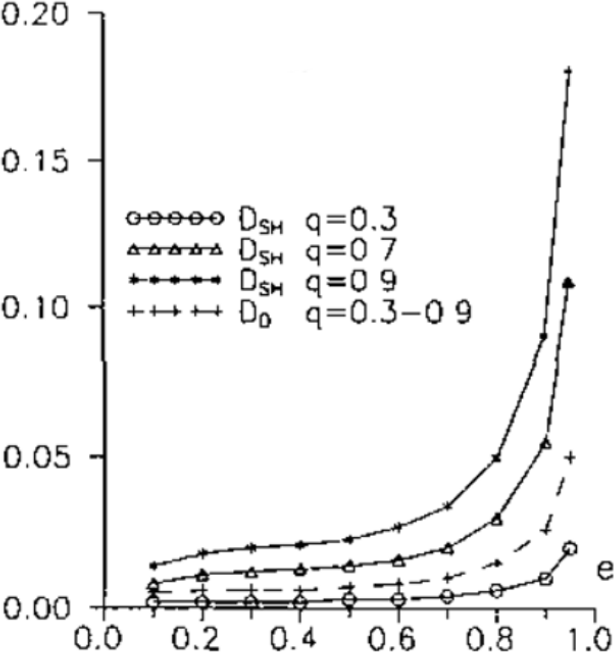
\includegraphics[width=0.4\linewidth]{img/plots/remarks-q.png}\label{img:revised:jopek:1}}\hfill
    \subfigure[excentricity $e$]{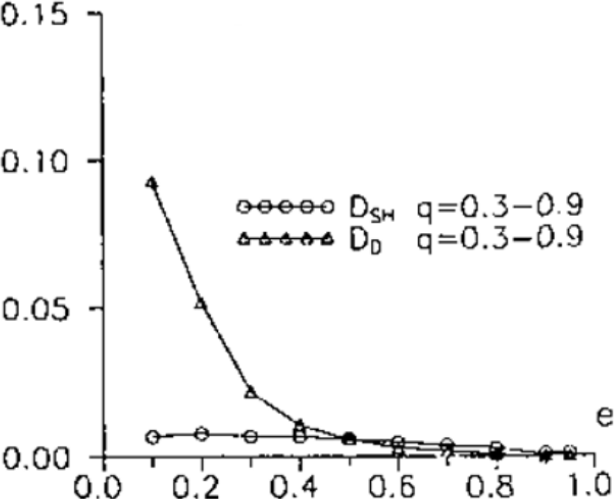
\includegraphics[width=0.4\linewidth]{img/plots/remarks-e.png}\label{img:revised:jopek:2}}
    \caption[Závislost členů $D$-kritérií na excentricitě]{
        Závislost členů $D$-kritérií na excentricitě\\
        {\small (zdroj: \cite{remarks})}
    }
    \label{img:revised:jopek}
\end{figure}

Cílem je, aby se příspěvek jednotlivých členů choval co nejvíce konstantě vzhledem k excentricitě. První, graf \ref{img:revised:jopek:1}, ukazuje, že $D_\text{SH}$ se příliš liší pro různé hodnoty $q$ a pro excentricity blízké jedné utíká do příliš vysokých hodnot. $D_\text{D}$ je v tomto ohledu stabilnější, tedy přidání váhy $1/(q_A+q_B)$ členu $(q_B-q_A)$ je zde přínosné. Naopak graf \ref{img:revised:jopek:2} ukazuje, že ve členu excentricit je mnohem stabilnější prostý rozdíl $(e_B-e_A)$ s váhou $1$ z funkce $D_\text{SH}$.

\medskip

Výsledkem této práce byla nová míra orbitální odlišnosti $D_\text{H}$, která je hybridem $D_\text{SH}$ a $D_\text{D}$ odstraňujícím vysokou citlivost obou měr na excentricitu \cite{remarks}. Tato míra má předpis \cite{remarks}
\begin{equation}
    \begin{aligned}
        D_\text{H}^2= & \left( \frac{q_B-q_A}{q_A+q_B} \right)^2                                    \\
                      & +\left( e_B-e_A \right)^2                                                   \\
                      & +\left( 2\sin{\frac{I_{AB}}{2}} \right)^2                                   \\
                      & +\left( \frac{e_A+e_B}{2} \right)^2\left( 2\sin{\frac{\Pi_{AB}}{2}} \right) \text{,}
    \end{aligned}
    \label{eqn:revised:d_h}
\end{equation}
kde $I_{AB}$ spočteme vzorcem \eqref{eqn:history:i_ba} a $\Pi_{AB}$ vzorcem \eqref{eqn:history:pi_ba}. Vhodnými hranicemi pro toto kritérium jsou \cite{galligan}
$$
    D_\text{H} \le \begin{cases}
        0{,}10 & i < 10^\circ \\
        0{,}16 & 10^\circ \le i < 90^\circ \text{.}
    \end{cases}
$$